\chapter{Marco colaborativo}

% obtener un clon digital, un problema especialmente complejo dadas las caracter\'isticas de los tejidos, que se conforman
% de una gran cantidad de elementos cuyas propiedades e interacciones entre s\'i determinan el aspecto final de la superficie

% llevar al sector textil un clon digital de los materiales y que permita a la industria beneficiarse de las ventajas de un
% proceso de produccion digital: velodidad de iteraci\'on, reducci\'on de costes, ubicuidad, menor coste medioambiental, etc.

Este proyecto educativo se desarrolla en estrecha colaboraci\'on con Seddi, empresa dedicada a la simulaci\'on gr\'afica que
trabaja en la creaci\'on de gemelos digitales de tejidos. La empresa cuenta con departamentos de investigaci\'on e ingenier\'ia para
crear un conjunto de soluciones que permitan a diferentes agentes de la industria textil, como empresas de manufactura, dise\~nadores,
patronistas o comerciales, trabajar y colaborar en tiempo real sobre una plataforma web.\\

Las tecnolog\'ias de digitalizaci\'on de Seddi se sustentan sobre los departamentos de investigaci\'on, que se dividen en dos grupos
seg\'un el tipo de propiedades a representar, \'opticas o mec\'anicas y que se corresponden con los departamentos de captura
\'optica y renderizado, y captura mec\'anica y simulaci\'on respectivamente.
El proceso de digitalizaci\'on comienza con la captura, en el que se utiliza la tecnolg\'ia desarrollada en los departamentos de captura
\'optica y mec\'anica para analizar muestras de tejido real, que luego se utilizar\'an en los modelos de simulaci\'on y renderizado
desarrollados en sendos departamentos para dar vida a la r\'eplicas digitales. 

\begin{figure}[H]
    \vspace{0.5cm}
    \centering
      \frame{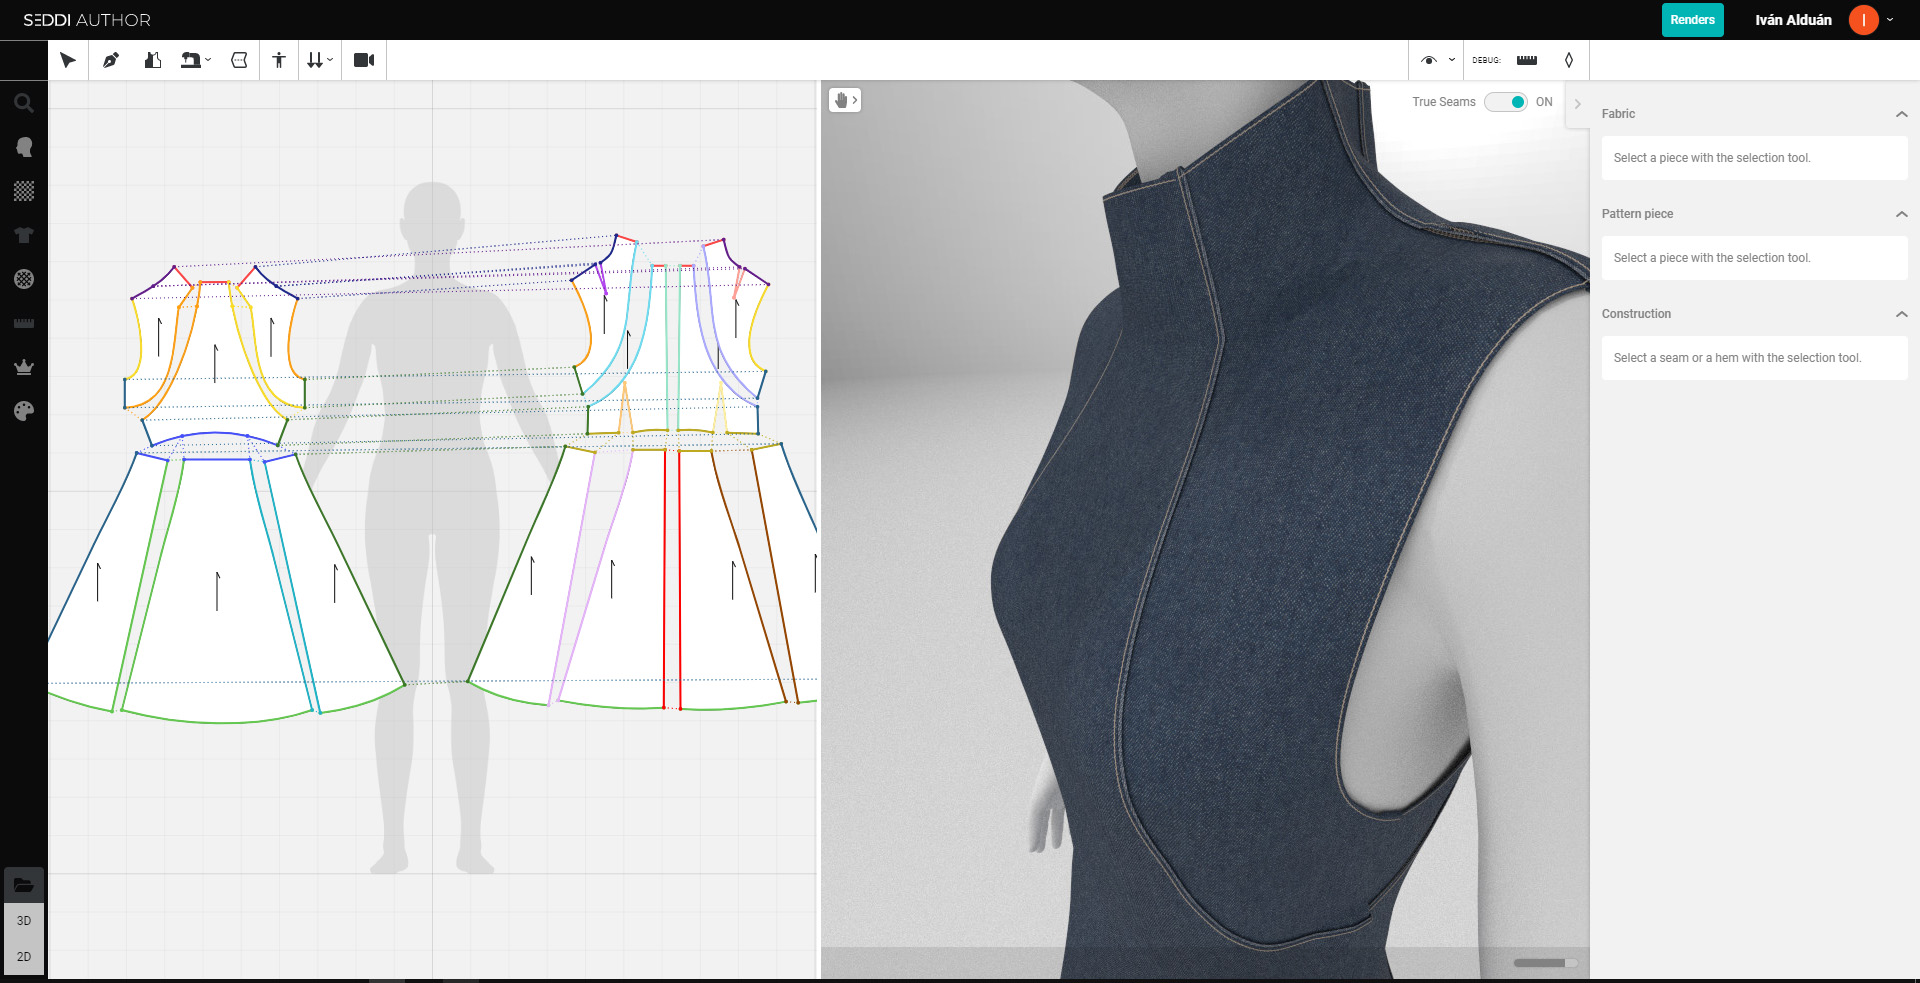
\includegraphics[scale=0.28]{seddicollaboration_ivan}}
    \caption[]{Vista de los entornos de trabajo 2D y 3D de Author}
\end{figure}
\newpage

Los departamentos de ingenier\'ia se encargan de crear la infraestructura e integrar las tecnolog\'ias desarrolladas en el \'area
de investigaci\'on para exponer su funcionalidad al usuario en las diferentes plataformas de Seddi.
Este Trabajo Fin de M\'aster (TFM) se enmarca bajo el contexto de Author, un departamento dentro del \'area de ingenier\'ia dedicado
a la creaci\'on de una plataforma que permita a los involucrados en el proceso de dise\~no, prototipado y construcci\'on de una prenda
trabajar y colaborar en una plataforma en la nube, utilizando las r\'eplicas digitales obtenidas durante el proceso de captura.\\

Author es una herramienta de edici\'on que permite importar, crear y editar patrones, definir los detalles constructivos de la prenda,
como el orden de costura, dobladillos, pinzas, etc., y ver en tiempo real una representaci\'on 3D realista del prototipo.
Para ello proporciona al usuario principalmente dos contextos de trabajo: un espacio 2D en el que trabajar el patronaje y detalles
de confecci\'on de la prenda, y un contexto 3D que permite previsualizar en tiempo real una simulaci\'on de la prenda sobre
un avatar digital. La previsualizaci\'on 3D es lo suficientemente precisa como para permitir trabajar con fluidez durante
el proceso de dise\~no, no obstante, para fases que requieran un mayor grado de realismo y detalle en la construcci\'on de la
prenda, se ofrece la posibilidad de utilizar los servicios de simulaci\'on y renderizado en la nube de Seddi para generar una
im\'agen de trazado de rayos renderizada progresivamente y transmitida en tiempo real al cliente web.\\

% La relaci\'on de colaboraci\'on establecida, brinda al alumno la oportunidad de desarrollo profesional bajo un proyecto formativo
% que ampl\'ia los conocimientos adquiridos durante el M\'aster en Computaci\'on Gr\'afica y Realidad Virtual de U-Tad
% y permite explorar nuevas t\'ecnicas para la visualizaci\'on hiperrealista de tejidos dentro del producto de Author.



% proporciona la capacidad se puede obtener una vista de la prenda con mayor grado de realismo que permita analizar en detalle
% los detalles de construcci\'on de la prenda utilizando los servicios de simulaci\'on renderizado en la nube de Seddi, 
% en la mayor\'ia de los casos

% con las
% ventajas
% trabajar con los clones digitales capturados previamente para crear prototipos realistas tanto en su aspecto visual como mec\'anico

%  colaborar a trav'\es de una herramientaen la nube

% una muestra de tejido y se obtienen datos
% sobre las propiedades mec\'anicas y \'opticas que determinan el movimiento y el aspecto de un tejido con las tecnolog\'ias
% desarrolladas en los departamentos de investigaci\'on en captura mec\'anica y \'optica. Una vez obtenidas
% las propiedades del modelo original, los algoritmos desarr


% Las tecnolog\'ias de digitalizaci\'on de Seddi se sustentan sobre los departamentos de investigaci\'on, que seg\'un su incidencia
% captura y simulaci\'on. El grupo captura, cuenta con departamentos de captura mec\'anica y captura \'optica, que se encargan
% de analizar muestras de tejidos y obtener los datos que determinan el movimiento y aspecto de un tejido en diferentes condiciones.

% \'opticas y mec\'anicas de la

% La tecnolog\'ia de Seddi se sustenta sobre los departamentos de investigaci\'on en captura \'optica y mec\'anica, que se encargan
% de analizar muestras de tejido y recoger datos sobre la interacci\'on de la luz sobre las fibras e informaci\'on sobre las propiedades
% que determina el movimiento de los tejidos, respectivamente, y los departamentos de renderizado y simulaci\'on, que desarrollan motores
% que utilizan los par\'ametros recogidos en la fase de captura para crear las representaciones digitales del modelo original.
% Por otra parte, los departamentos de ingenier\'ia de Seddi se encargan de integrar y exponer estas funcionalidades al usuario a trav\'es
% de una infraestructura de servicios en la nube.\\

% Estas tecnolog\'ias se proveen a los usuarios a trav\'es de una infraestructura de servicios web desarrollada
% por los departamentos de ingenier\'ia, que se encargan de desarrollar aplicaciones que exponen al usuario

% , que se especializan en la captura y simulaci\'on
% de las propiedades \'opticas y mec\'anicas de un tejido, cuyas aplicaciones se ofrecen a trav\'es de una infraestructura de
% servicios desarrollada por los departamentos de ingenier\'ia. 

% Los tejidos tiene una problem\'atica asociada, la cantidad de elementos y la interacci\'on entre ellos que resultan determinantes
% en el aspecto final del material; propiedades como el brillo o la ca\'ida de una prenda son el fruto de \'estas interacciones.

% determinan el aspecto final del material, por lo que
% son superficies especialmente dif\'iciles de simular, tanto a nivel \'optico como mec\'anico. 

% Seddi es una startup nacida como fruto de la investigacion en tecnologias de simulacion optica y mecanica aplicadas al sector textil.
% Propone ofrecer una solucion digital que permita a los disenhadores, patronistas o comerciales trabajar en un entorno colaborativo que
% representa con gran fidelidad los elementos constructivos de un prenda de ropa: tejido, costuras, dobladillos, etc.

% La caida, el brillo y, en general, la apariencia de una prenda son factores clave para validar o rechazar el producto, estas caracteristicas
% dependen de propiedades opticas y mecanicas que las herramientas de disenho actuales no tienen en cuenta, por lo que los profesionales del
% sector no satisfacen las necesidades de los profesionales de la industria, que en la mayor parte de los casos mantienen un proceso de
% trabajo artesanal en el que el prototipado y construccion de la prenda es un proceso iterativo entre patronista y disenhador y cuyo
% resultado depende en gran medida de la experiencia y destreza de estos profesionales.\\

% Para ofrecer su solucion, Seddi cuenta con departamentos de investigacion simulacion y captura tanto mecanica como optica, que desarrollan
% nuevos algoritmos y hardware que permitan un mayor grado de fidelidad en el momento de captura de los parametros que conforman la apariencia
% de una prenda, tanto como mejorar su representacion digital asi como departamentos de desarrollo de producto, se encargan del proceso de
% captura utilizando estas tecnologias propietarias asi como de integrar estos algoritmos en diferentes plataformas que permitan al consumidor
% final interactuar sobre los tejidos digitales durante diferentes etapas asociadas a este proceso de produccion con el fin de facilitar,
% acelerar y reducir los costes de produccion.

% Para conseguir un resultado fidedigno, en Seddi, el proceso comienza creando un clon digital del tejido, la obtencion de parametros opticos y
% mecanicos que identifican el tejido y se valida utilizando las tecnologias de simulacion y render de la empresa. 

% Todos las herramientas de Seddi se alojan en la nube, lo que garantiza disponibilidad inmediata a los recursos a todo el equipo involucrado en
% el proceso de produccion. Estos equipos, con un negocio de la moda cada dia mas globalizado, pueden tratarse de equipos multidisciplinares de
% diferentes empresas o paises, por lo que es primordial un flujo de comunicacion constante que minimice los errores y los costes economicos y
% medioambientales de los flujos de disenho y prototipado

% Gracias a esta estrategia de implementación, el contenido diseñado está disponible de manera inmediata y editable en un escenario global. En la
% actualidad, el negocio de la moda está completamente globalizado, y las tareas de diseño y prototipado de muchas marcas se hacen entre equipos
% internacionales o mediante subcontratación entre empresas. La  utilización de las soluciones cloud de Seddi permitirá a los equipos colaborar remotamente sobre un mismo diseño.
% En Seddi, el proceso para llegar a construir una prenda, comienza con la digitalizacion de un tejido, que se consigue a partir de muestras que
% son analizadas por maquinas de captura desarrolladas en Seddi, para obtener los parametros mecanicos y opticos
